\documentclass{article}
\usepackage{mathtools}
\usepackage{amsfonts}
\usepackage[utf8]{inputenc}

\newtheorem{definition}{Definice}
\newtheorem{proposition}{Tvrzení}
\newtheorem{theorem}{Věta}
\newtheorem{lemma}{Lemma}
\def\qed{{\hfill{$\square$}}}

\begin{document}

%poznámka: k v pk a sk má být velké

\section{Collision-Resistant Hash functions (CRHF's)}
Pro podpis libovolně dlouhé zprávy nejprve aplikujeme hash $h$ a pak až digitální podpis.
Požadavky:
\begin{itemize}
\item Výstup $h$ je ostře menší než vstup: $|h(m)| << |m|$.
\item Funkce $h$ je efektivně spočitatelná.
\item Je těžké efektivně nalézt kolizi: $(m,m'): m\neq m'$ a $h(m) = h(m')$.
\end{itemize}

\begin{definition}
$H = \bigl\{h_i: \{0,1\}^{\ell_d(i)} \to \{0,1\}^{\ell_r(i)} \bigr\}_{i \in I}$
je \emph{kolekcí CRHF's} pokud platí:
\begin{enumerate}
\item Generování: existuje PPT $G: i \leftarrow G(1^n), i \in I$.
\item Komprese: $\ell_d(i) > \ell_r(i), \forall i \in I$.
\item Efektivita: $h_i(x)$ lze vyhodnotit v čase $\textit{poly}(i)$ pro všechny $i \leftarrow G(1^n)$ a $x \in \{0,1\}^{\ell_d(i)}$.
\item Collision Resistent: Pro všechny PPT $A$ existuje negligible funkce $\varepsilon$ taková, že
\[
\Pr[A(i) = (x,x'): x \neq x', h_i(x) = h_i(x')] \leq \varepsilon(n),
\]
kde pravděpodobnost je přes $i \leftarrow G(1^n)$ a náhodné mince $A$.
\item Technická podmínka: $n \leq \textit{poly}(i)$ pro všechny $i \leftarrow G(1^n)$.
\end{enumerate}
\end{definition}

\begin{itemize}
\item Typické nastavení: $\ell_d(i)$ je libovolné a $\ell_r(i) = n$.
\item Možné útoky:
\begin{enumerate}
\item Hádání: $\ell_d = 2n$ a $\ell_r = n$.
\begin{itemize}
\item Vybereme náhodně $m,m' \leftarrow \{0,1\}^{2n}$ $\bigl(\Pr[m = m'] = \frac{1}{2^{2n}}\bigr)$.
\item Kolizi uhádneme s pravděpodobností vyšší než $\frac{1}{2^n} - \frac{1}{2^{2n}}$.
\end{itemize}
\item Birthday Attack:
\begin{itemize}
\item Vybereme $t$ náhodných zpráv a hledáme kolizi.
\item Pravděpodobnost, že najdeme kolizi je počet dvojic krát pravděpodobnost kolize v náhodné dvojici. Tedy pravděpodobnost nalezení kolize je větší než:
\[
\binom{t}{2} \Bigl(\frac{1}{2^n} - \frac{1}{2^{2n}}\Bigr) \approx \frac{t^2}{2^{n+1}}.
\]
\item Pro $t = \Theta\bigl(2^{\frac{n}{2}}\bigr)$ pak máme konstantní pravděpodobnost nalezení kolize.
\end{itemize}
\end{enumerate}
\end{itemize}

\section{Universal One-way Hash Functions}
\noindent Collision-resistent je silný předpoklad, někdy stačí následující:
\begin{enumerate}
\item $A$ zvolí $x \in \{0,1\}^{\ell_d(i)}$.
\item $i \leftarrow G(1^n)$.
\item $A$ vrátí $x': x \neq x'$ a $h_i(x) = h_i(x')$.
\end{enumerate}
\begin{itemize}
\item UOWHF's existují pokud existují jednosměrné funkce.
\item CRHF's nelze zkonstruovat pomocí black-box metod ani z jednosměrných permutací.
\end{itemize}

\section{Merkle-Damgård Transformace}
\noindent Definice CRHF's dává kompresi o 1 bit, nyní ukážeme kompresi o libovolný počet bitů.
\begin{enumerate}
\item Kompresní funkce $h: \{0,1\}^{\ell + n} \to \{0,1\}^n$.
\item Pro zprávu $M \in \{0,1\}^*$:
\begin{enumerate}
\item Rozděl $M$ do bloků délky $\ell$:
\[
M = M_1 || M_2 || M_3 || \dots || M_t.
\]
Blok $M_t$ je doplněn 0 na délku $\ell$.
Definujme funkci $H$ následovně
\[
H(M) = h\Bigl(M_t || h\bigl(M_{t-1} || h(M_{t-2} \dots h(M_1 || IV) \dots)\bigr)\Bigr),
\]
kde $IV$ je inicializační vektor nastaven například na samé 0.
\end{enumerate}
\end{enumerate}
Schéma transformace je zobrazeno na následujícím obrázku.
\begin{figure}[h]
\centering
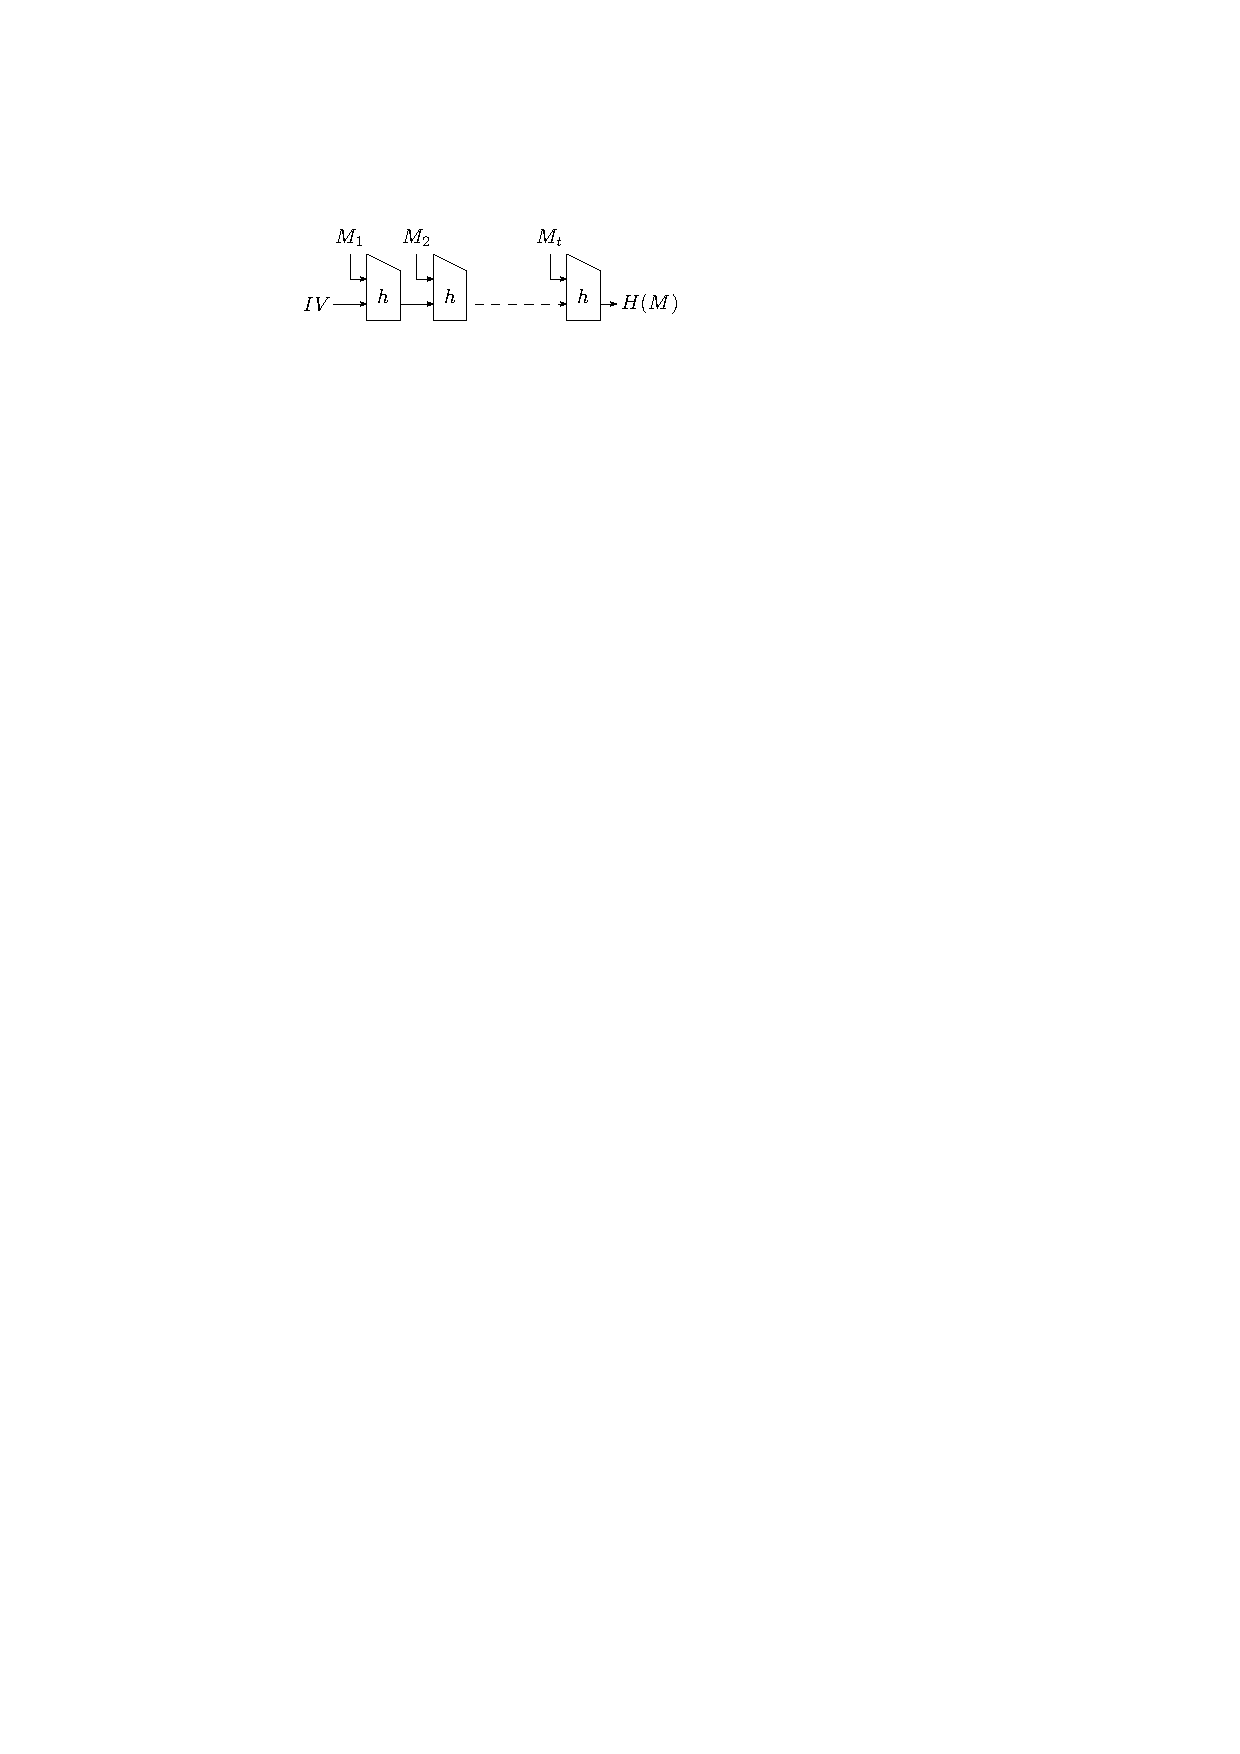
\includegraphics{MD_transformace.pdf}
\end{figure}
\begin{proposition}
Pokud je $h$ kolekcí CRHF's pak i $H$ je kolekcí CRHF's.
\end{proposition}

\section{Konstrukce CRHF's}
\begin{theorem}
Kolekce CRHF's existují pokud platí předpoklad o obtížnosti faktorizace přirozených čísel nebo nalezení diskrétního logaritmu.
\end{theorem}
\noindent{\it Myšlenka důkazu.}
Mějme generátor $g$ pro grupu $\mathbb{Z}_p^*$.
Nechť $y \leftarrow \mathbb{Z}_p^*$.
Problém diskrétního logaritmu je nalézt $x \in \mathbb{Z}_{p-1}$ takové, že $g^x \equiv y~(mod~p)$.
Definujme
\begin{align*}
h_{p,g,y}&: \mathbb{Z}_{p-1} \times \{0,1\} \to \mathbb{Z}_p^*, \\
h_{p,g,y}&(x,b) = y^b \cdot g^x~(mod~p).
\end{align*}
Ukážeme, že kolize $h_{p,g,y}$ nám dává diskrétní logaritmus $y$.
Mějme PPT $A$, který najde s velkou pravděpodobností kolizi $(x,b) \neq (x',b')$ a $h_{p,g,y}(x,b) = h_{p,g,y}(x',b')$.
Rozlišíme dva případy. 
Předpokládejme, že $b = b'$, pak ukážeme, že nenastane kolize.
Pokud $y^b \cdot g^x \equiv y^b g^{x'}~(mod~p)$, pak také $g^x \equiv g^{x'}~(mod~p)$.
Prvek $g$ je ale generátor grupy $\mathbb{Z}_p^*$, tedy $x = x'$.

Nechť tedy $b \neq b'$ a bez újmy na obecnosti $b = 0$ a $b' = 1$.
Pak tedy máme
\begin{align*}
g^x &\equiv y g^{x'}~(mod~p) \\
y &\equiv g^{x - x'}~(mod~p).
\end{align*}
Tedy $x - x'$ je diskrétní logaritmus $y$ vzhledem ke $g$.
\qed

\section{Hashovací Funkce v Praxi}
\begin{center}
\begin{tabular}{|ccccl|}
\hline
{\bf Schéma} & {\bf Návrh} & {\bf Délka Výstupu} & {\bf Útok} & {\bf Poznámka} \\
& & (v bitech) & & \\
\hline
MD4 & Rivest, 1990 & 128 & 1995 & \\
\hline
MD5 & 1992 & 128 & 1998 & \\
\hline
SHA1 & 1994 & 160 & 2005 & \textbullet~Kolize v čase $2^{60}$ \\
& & & & \textbullet~Lepší než birthday attack \\
\hline
SHA2/SHA256 & 2005 & 256 & Zatím neprolomen & \textbullet~Heuristický kandidát \\
& & & & \textbullet~Používá se v bitcoinu \\
\hline
\end{tabular}
\end{center}

\section{Hash-then-Sign}
Nyní ukážeme, že pokud existují kolekce CRHF's pak existují schémata elektronického podpisu pro libovolně dlouhé zprávy.
Nechť $(G,S,V)$ je one-time elektronický podpis pro ${\sc M} = \{0,1\}^n$ a $H$ je kolekcí CRHF's pro $\{0,1\}^*$ s výstupy délky $n$.
Zkonstruujeme one-time elektronický podpis $(G',S',V')$ pro zprávy libovolné délky.
\begin{description}
\item[$G'$:] $pk'=(pk,i), sk'=(sk,i)$, kde $(pk,sk) \leftarrow G(1^n)$ a pro generátor $G_H$ z $H$: $i \leftarrow G_H(1^n)$.
\item[$S'$:] $S'_{sk}(m) = S_sk\bigl(h_i(m)\bigr)$.
\item[$V'$:] $V'_{pk}(m,\sigma) = V_{pk}\bigl(h_i(m),\sigma\bigr)$.
\end{description}

\begin{theorem}
Pokud $(G,S,V)$ je secure one-time elektronický podpis pro ${\sc M} = \{0,1\}^n$ a $H$ je kolekce CRHF's pro $\{0,1\}^*$ pak $(G',S',V')$ je secure one-time elektronický podpis pro ${\sc M}' = \{0,1\}^*$.
\end{theorem}
\noindent\textit{Důkaz.}
Mějme PPT $A$, který padělá podpis pro $(G',S',V')$ s pravděpodobností alespoň $\varepsilon$ (non-negligible).
Algoritmus $A(pk')$ pošle nejvýše jeden dotaz $m$ na $S'_{sk'}(\cdot)$ a dostane odpověď $\sigma' \leftarrow S'_{sk'}(m)$.
Algoritmus $A$ uspěje pokud vrátí $(m',\sigma')$ takové, že $m \neq m'$ a $V'_{pk'}(m',\sigma') = \textit{accept}$.

\section{Další Aplikace CRHF's}
\begin{itemize}
\item Fingerprinting
\item Deduplikace dat -- test, zda soubor již není na serveru
\end{itemize}
\subsection{Merkle Hash Tree}
Mějme $h: \{0,1\}^{2\ell} \to \{0,1\}^\ell$ a data $X = \{0,1\}^*$. 
Rozdělíme $X$ do bloků velikosti $\ell$, tedy
\[
X = x_1 || x_2 || \dots || x_t,
\]
kde $|x_i| = \ell$.
Můžeme předpokládat, že $|X| = \ell t$ a $t$ je mocnina 2, jinak použijeme padding nulami.
Mějme binární strom s $t$ listy.
Ke každému vrcholu $v$ přiřadíme hodnotu $c_X(v) \in \{0,1\}^\ell$.
Do listů umístíme bloky $x_i$ a následně počítáme hashe od listu nahoru.
Mějme vrchol $v$ jehož synové $v_1$ a $v_2$ již mají spočítané hodnoty $c(v_1)$ a $c(v_2)$ pak hodnota na vrcholu $v$ bude $c_X(v) = h\bigl(c_X(v_1) || c_X(v_2)\bigr)$. 
Označme $MT_h(X)$ hodnotu v kořeni stromu.

Příklad použití: chceme uložit data na serveru a mít možnost ověřit, že server data nezměnil bez toho aniž bychom si daná data pamatovali.
\begin{enumerate}
\item Spočítáme $MT_h(X)$ a odešleme data na server.
\item Chceme získat $x_i$ a ověřit, že server data nezměnil.
\item Nechť $P$ je cesta z listu, kde je uloženo $x_i$, do kořene stromu.
\item Server pošle hodnoty všech vrcholů z $P$ a všech jejich bratrů.
\item Nyní můžeme ověřit, zda hodnoty na cestě $P$ jsou správně spočítané a zda hodnota v kořeni je rovna $MT_h(X)$ -- je potřeba $O(\log t)$-krát spočítat $h$.
\item Aby server podvrhl $x_i$ musí umět nalézt kolizi $h$.
\end{enumerate}

\begin{figure}
\centering
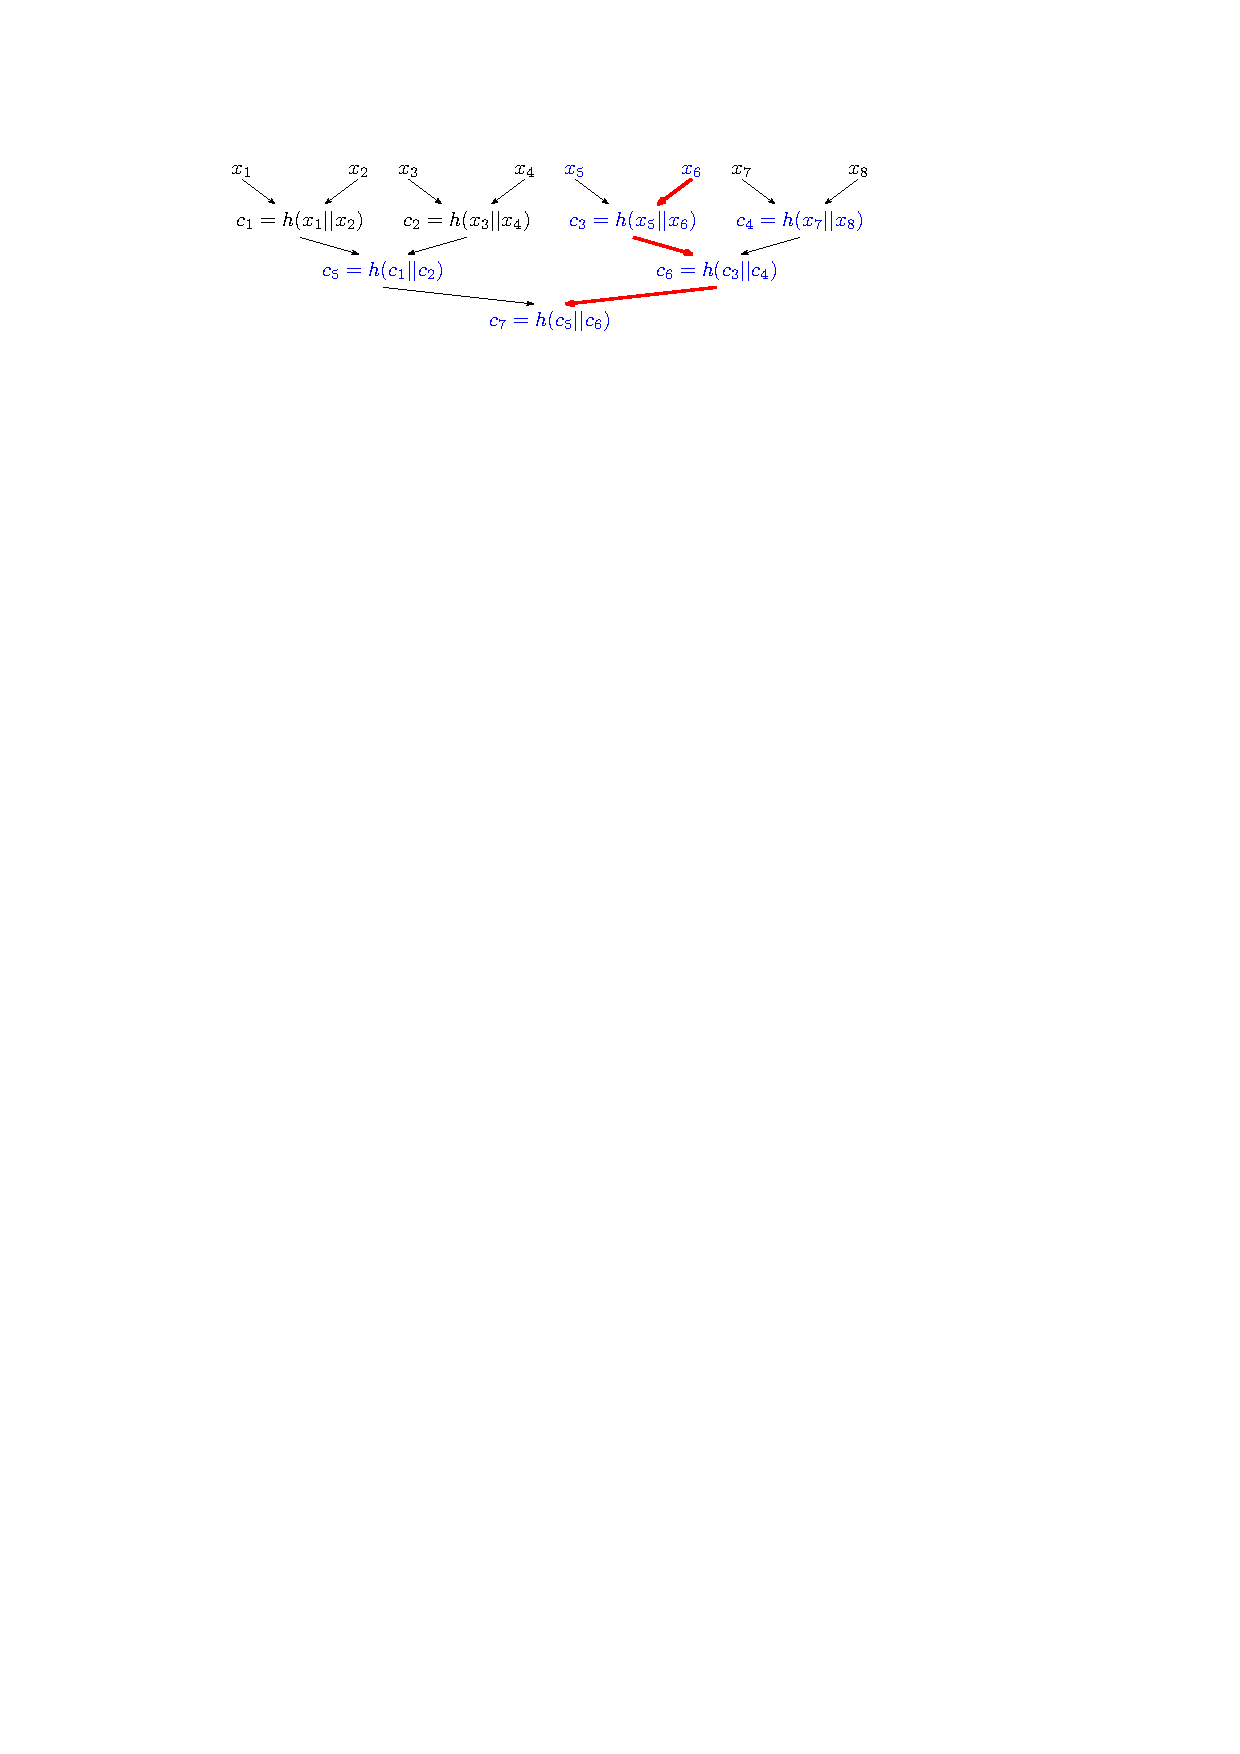
\includegraphics{hash_tree.pdf}
\caption{Příklad Merkle hash tree pro data s 8 bloky. Při vyžádání bloku $x_6$ ze serveru je červeně vyznačená cesta $P$ z listu $x_6$ do kořene a modře jsou označeny data, která server odešle.}
\end{figure}
\begin{lemma}
Nechť $MT_h(X) = MT_h(X')$ pro $X \neq X' \in \{0,1\}^{t\ell}$. 
Pak musí existovat vrchol $v$ ve stromu se syny $v_1$ a $v_2$ takový, že 
\begin{align*}
c_X(v_1) || c_X(v_2) &\neq c_{X'}(v_1) || c_{X'}(v_2), \\
h\bigl(c_X(v_1) || c_X(v_2)\bigr) &= h\bigl(c_{X'}(v_1) || c_{X'}(v_2)\bigr).
\end{align*}
\end{lemma}
\noindent\textit{Důkaz.}
Postupujme od listů nahoru.
Mějme $x_i$ a $x'_i$ bloky $X$ a $X'$ takové, že $x_i \neq x'_i$.
Vezměme list $v_1$, kde jsou uloženy $x_i$ a $x'_i$ a jeho bratra $v_2$.
Pro vrcholy $v_1$ a $v_2$ jistě platí, že
\[
c_X(v_1) || c_X(v_2) \neq c_{X'}(v_1) || c_{X'}(v_2).
\]
Nechť $v$ je jejich otec.
Pokud pro $v$ platí, že $c_X(v) = c_{X'}(v)$, pak jsme skončili.
Jinak vezmeme $v_1 := v$ a $v_2$ je bratr $v$ a celý proces opakujeme.
Jelikož pro kořen stromu $r$ platí, že $c_X(r) = c_{X'}(r)$ tak jistě najdeme požadované vrcholy $v$, $v_1$ a $v_2$.
\end{document}
